\chapter{Análisis para $Q = \num{0.25}$}
\label{chap:q025}

\section{Función de transferencia}

Con $R = \qty{100}{\ohm}$, $L = \qty{37.31}{\milli\henry}$ y $C = \qty{59.70}{\micro\farad}$, los
coeficientes de la ecuación~\eqref{eq:tf-componentes} resultan

\begin{gather*}
  \frac{R}{L} = \frac{\qty{100}{\ohm}}{\qty{37.31}{\milli\henry}} = \num{2680.25}, \qquad
  \frac{1}{LC} = \frac{1}{\qty{37.31}{\milli\henry} \cdot \qty{59.70}{\micro\farad}} = \num{448952.5},
\end{gather*}

por lo que la función de transferencia del filtro es

\begin{equation}
  H_1(s) = \frac{s^2}{s^2 + \num{2680.25}\, s + \num{448952.5}}
         = \frac{s^2}{\left(s + \num{179.53}\right)\left(s + \num{2500.72}\right)}.
  \label{eq:tf-q025}
\end{equation}

\section{Raíces y lugar de raíces}

El polinomio característico tiene discriminante positivo
($\num{2680.25}^2 - 4 \cdot \num{448952.5} > 0$), de modo que sus raíces son reales y distintas:

\begin{gather*}
  s_1 = \num{-179.53}\ \unit{\radian\per\second}, \qquad
  s_2 = \num{-2500.72}\ \unit{\radian\per\second},
\end{gather*}

a las que se suma el cero doble en el origen. La Figura~\ref{fig:polos-q025} muestra su ubicación en el
plano complejo: ambos polos se encuentran sobre el semieje real negativo, uno de ellos
($s_1$, equivalente a \qty{28.6}{\hertz}) mucho más cercano al origen que el otro
($s_2$, equivalente a \qty{398}{\hertz}). El polo $s_2$ es el que fija en la práctica la frecuencia de corte,
mientras que $s_1$ es el polo dominante de la respuesta temporal.

\begin{figure}[!ht]
  \centering
  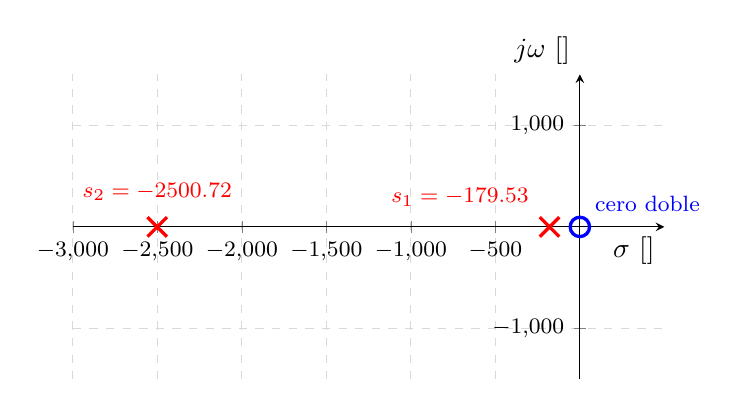
\begin{tikzpicture}
  \begin{axis}[
    width=0.75\textwidth, height=0.45\textwidth,
    axis lines=middle,
    xlabel={$\sigma$ [\unit{\radian\per\second}]},
    ylabel={$j\omega$ [\unit{\radian\per\second}]},
    xlabel style={at={(ticklabel* cs:1)}, anchor=north east},
    ylabel style={at={(ticklabel* cs:1)}, anchor=south east},
    xmin=-3000, xmax=500, ymin=-1500, ymax=1500,
    xtick={-3000,-2500,-2000,-1500,-1000,-500},
    ytick={-1000,1000},
    grid=both, grid style={gray!30, dashed},
    tick label style={font=\footnotesize},
    clip=false,
  ]
    \addplot[only marks, mark=x, mark size=5pt, very thick, red]
      coordinates {(-2500.72,0) (-179.53,0)};
    \addplot[only marks, mark=o, mark size=3.5pt, very thick, blue] coordinates {(0,0)};
    \node[above=6pt, red, font=\footnotesize] at (axis cs:-2500.72,0) {$s_2 = \num{-2500.72}$};
    \node[above left=4pt, red, font=\footnotesize] at (axis cs:-179.53,0) {$s_1 = \num{-179.53}$};
    \node[above right=2pt, blue, font=\footnotesize] at (axis cs:0,0) {cero doble};
  \end{axis}
\end{tikzpicture}

  \caption{Ubicación de polos y ceros de $H_1(s)$ en el plano complejo.}
  \label{fig:polos-q025}
\end{figure}

\section{Factor de amortiguamiento}

De la ecuación~\eqref{eq:xi},

\begin{equation}
  \xi = \frac{1}{2Q} = \frac{1}{2 \cdot \num{0.25}} = 2,
  \label{eq:xi-q025}
\end{equation}

valor mayor que la unidad y coherente con las dos raíces reales distintas halladas. La constante de
corrección de la frecuencia de corte para este caso es $K = \num{0.2666}$, lo que indica que la pulsación
natural $\omega_0 = \qty{670.0}{\radian\per\second}$ se encuentra muy por debajo de la de corte.

\section{Respuesta temporal}

Se analiza la respuesta ante un escalón unitario, $v_i(t) = u(t)$, cuya transformada es
$V_i(s) = 1/s$. La salida en el dominio de Laplace es entonces

\begin{equation}
  V_o(s) = H_1(s)\, V_i(s)
         = \frac{s}{\left(s + \num{179.53}\right)\left(s + \num{2500.72}\right)}
         = \frac{A}{s + \num{179.53}} + \frac{B}{s + \num{2500.72}}.
  \label{eq:vo-q025}
\end{equation}

Igualando numeradores, $A\left(s + \num{2500.72}\right) + B\left(s + \num{179.53}\right) = s$, lo que
conduce al sistema $A + B = 1$ y $\num{2500.72}\,A + \num{179.53}\,B = 0$. Resolviendo:

\begin{gather*}
  A = \frac{\num{-179.53}}{\num{2500.72} - \num{179.53}} = \num{-0.07734}, \qquad
  B = \frac{\num{2500.72}}{\num{2500.72} - \num{179.53}} = \num{1.07734}.
\end{gather*}

Antitransformando término a término se obtiene la respuesta temporal

\begin{equation}
  v_o(t) = \left(\num{1.07734}\, e^{-\num{2500.72}\, t} - \num{0.07734}\, e^{-\num{179.53}\, t}\right) u(t),
  \label{eq:vo-t-q025}
\end{equation}

que se grafica en la Figura~\ref{fig:escalon-q025}. En $t = 0^+$ la salida reproduce íntegramente el salto
de entrada ($v_o(0^+) = A + B = 1$), ya que el capacitor se comporta como un cortocircuito y el inductor
como un circuito abierto frente al flanco. Luego la salida decae hacia cero: el término rápido se extingue
en pocas décimas de milisegundo y el término lento, de signo negativo, provoca un pequeño paso por valores
negativos antes de alcanzar el valor final.

\begin{figure}[!ht]
  \centering
  \begin{tikzpicture}
  \begin{axis}[
    name=principal,
    width=0.9\textwidth, height=0.55\textwidth,
    xlabel={$t$ [\unit{\milli\second}]}, ylabel={Tensión [\unit{\volt}]},
    xmin=0, xmax=12, ymin=-0.1, ymax=1.1,
    grid=both, grid style={gray!30, dashed},
    legend pos=north east, legend cell align=left, legend style={font=\footnotesize},
    tick label style={font=\footnotesize},
    samples=400, domain=0:12, no marks,
  ]
    \addplot[gray, thick, dotted] {1};
    \addlegendentry{$v_i(t)$ (escalón unitario)}
    \addplot[blue, very thick] {1.07734*exp(-2.50072*x) - 0.07734*exp(-0.17953*x)};
    \addlegendentry{$v_o(t)$ para $Q = \num{0.25}$}
    \addplot[red, dashed] {0.02};
    \addlegendentry{banda de $\pm\qty{2}{\percent}$}
    \addplot[red, dashed, forget plot] {-0.02};
    \draw[dashed, gray] (axis cs:7.53,-0.1) -- (axis cs:7.53,0.08);
  \end{axis}
  % detalle ampliado de la zona del subpico
  \begin{axis}[
    at={(principal.north east)}, anchor=north east, xshift=-0.6cm, yshift=-2.0cm,
    width=0.5\textwidth, height=0.28\textwidth,
    xmin=0, xmax=12, ymin=-0.07, ymax=0.04,
    ytick={-0.06,-0.04,-0.02,0,0.02},
    scaled y ticks=false,
    yticklabel style={/pgf/number format/fixed, /pgf/number format/precision=2},
    grid=both, grid style={gray!30, dashed},
    tick label style={font=\scriptsize},
    axis background/.style={fill=white},
    samples=400, domain=0:12, no marks,
  ]
    \addplot[blue, very thick] {1.07734*exp(-2.50072*x) - 0.07734*exp(-0.17953*x)};
    \addplot[red, dashed] {0.02};
    \addplot[red, dashed] {-0.02};
    \addplot[only marks, mark=*, mark size=1.5pt, black] coordinates {(2.269,-0.0478)};
    \node[below right=1pt, font=\scriptsize] at (axis cs:2.269,-0.0478)
      {subpico \qty{-4.8}{\percent} en $t = \qty{2.27}{\milli\second}$};
    \draw[dashed, gray] (axis cs:7.53,-0.07) -- (axis cs:7.53,0.04)
      node[pos=0.72, right, font=\scriptsize, black] {$t_s = \qty{7.53}{\milli\second}$};
    \node[anchor=north west, font=\scriptsize\itshape] at (rel axis cs:0.02,0.98) {detalle};
  \end{axis}
\end{tikzpicture}

  \caption{Respuesta al escalón unitario del filtro con $Q = \num{0.25}$.}
  \label{fig:escalon-q025}
\end{figure}

\section{Parámetros de la respuesta temporal}

Dado que la respuesta al escalón de un filtro pasa alto parte del valor del salto y evoluciona hacia cero,
los parámetros clásicos de los sistemas de segundo orden se adaptan de la siguiente manera: el tiempo de
crecimiento se reemplaza por el tiempo de caída entre el \qty{90}{\percent} y el \qty{10}{\percent} del
salto inicial; el sobrepico se mide como la máxima excursión por debajo del valor final (subpico),
referida al salto inicial; y el tiempo de establecimiento es el instante a partir del cual la salida
permanece dentro de una banda de $\pm\qty{2}{\percent}$ del salto alrededor del valor final. Los valores
medidos sobre la ecuación~\eqref{eq:vo-t-q025} se resumen en la Tabla~\ref{tab:parametros-q025}.

\begin{table}[!ht]
  \centering
  \begin{tabular}{|l|c|}
    \hline
    Parámetro & Valor \\
    \hline
    Valor inicial $v_o(0^+)$                              & \qty{1}{\volt} \\
    Tiempo de caída (\qty{90}{\percent} a \qty{10}{\percent}) & \qty{0.70}{\milli\second} \\
    Subpico máximo                                        & \qty{-4.8}{\percent} \\
    Instante del subpico                                  & \qty{2.27}{\milli\second} \\
    Tiempo de establecimiento (\qty{2}{\percent})         & \qty{7.53}{\milli\second} \\
    Constante de tiempo dominante $\tau_1 = 1/|s_1|$      & \qty{5.57}{\milli\second} \\
    \hline
  \end{tabular}
  \caption{Parámetros de la respuesta al escalón para $Q = \num{0.25}$.}
  \label{tab:parametros-q025}
\end{table}

El tiempo de establecimiento queda determinado casi exclusivamente por el polo dominante: a partir de la
ecuación~\eqref{eq:vo-t-q025}, despreciando el término rápido, la salida ingresa definitivamente en la
banda del \qty{2}{\percent} cuando $\num{0.07734}\, e^{-t/\tau_1} = \num{0.02}$, es decir, en
$t_s = \tau_1 \ln\left(\num{0.07734}/\num{0.02}\right) = \qty{7.53}{\milli\second}$, en coincidencia con el
valor medido.

\section{Tipo de amortiguamiento}

Con $\xi = 2 > 1$ y dos raíces reales distintas, el filtro es sobreamortiguado. La respuesta no presenta
oscilaciones: la salida decae de forma monótona hasta un único subpico de muy baja amplitud
(\qty{-4.8}{\percent}) y luego retorna lentamente a cero, gobernada por la constante de tiempo del polo
más cercano al origen.
